\section{Frontend}\label{sec:visualisierung-im-frontend}

Das Frontend des Evaluationsframeworks setzt die Anforderungen \hyperlink{FA05}{FA05} und \hyperlink{FA06}{FA06} um. Es unterstützt die interaktive Konfiguration von Evaluierungen, die Live-\linebreak~Verfolgung des Fortschritts sowie die detaillierte Analyse der Ergebnisse bis auf Ebene einzelner Testfälle. Die Oberfläche ist so gestaltet, dass zentrale Kennzahlen wie Accuracy, Precision, Recall und F1-Score, die Konfusionsmatrix mit \ac{TP}, \ac{FP}, \ac{TN}, \ac{FN} sowie die Bestehensraten aller Modelle zunächst auf einen Blick erfasst und anschließend schrittweise vertieft werden können.

\subsection*{Konfigurationsansicht}

Abbildung \ref{fig:evaluation-config} zeigt das Formular zur Konfiguration einer Evaluierung. Sämtliche Parameter, die bereits aus der YAML-Konfiguration in Kapitel \ref{sec:konfiguration-einer-evaluierung} bekannt sind, lassen sich hier setzen. Verfügbare Standardwerte, zum Beispiel der Endpunkt der in dieser Arbeit verwendeten Klassifizierungspipeline oder die in der Datenbank verfügbaren Datensätze, werden automatisch geladen.

YAML-Konfigurationen können importiert und exportiert werden, um sie zu speichern oder weiterzugeben. Unter dem Formular befinden sich Schaltflächen zum Starten der Evaluierung sowie zum Import und Export von JSON-Berichten. Auf diese Weise lassen sich Ergebnisse archivieren und später erneut laden, ohne die Evaluierung erneut ausführen zu müssen.

\begin{figure}
    \centering
    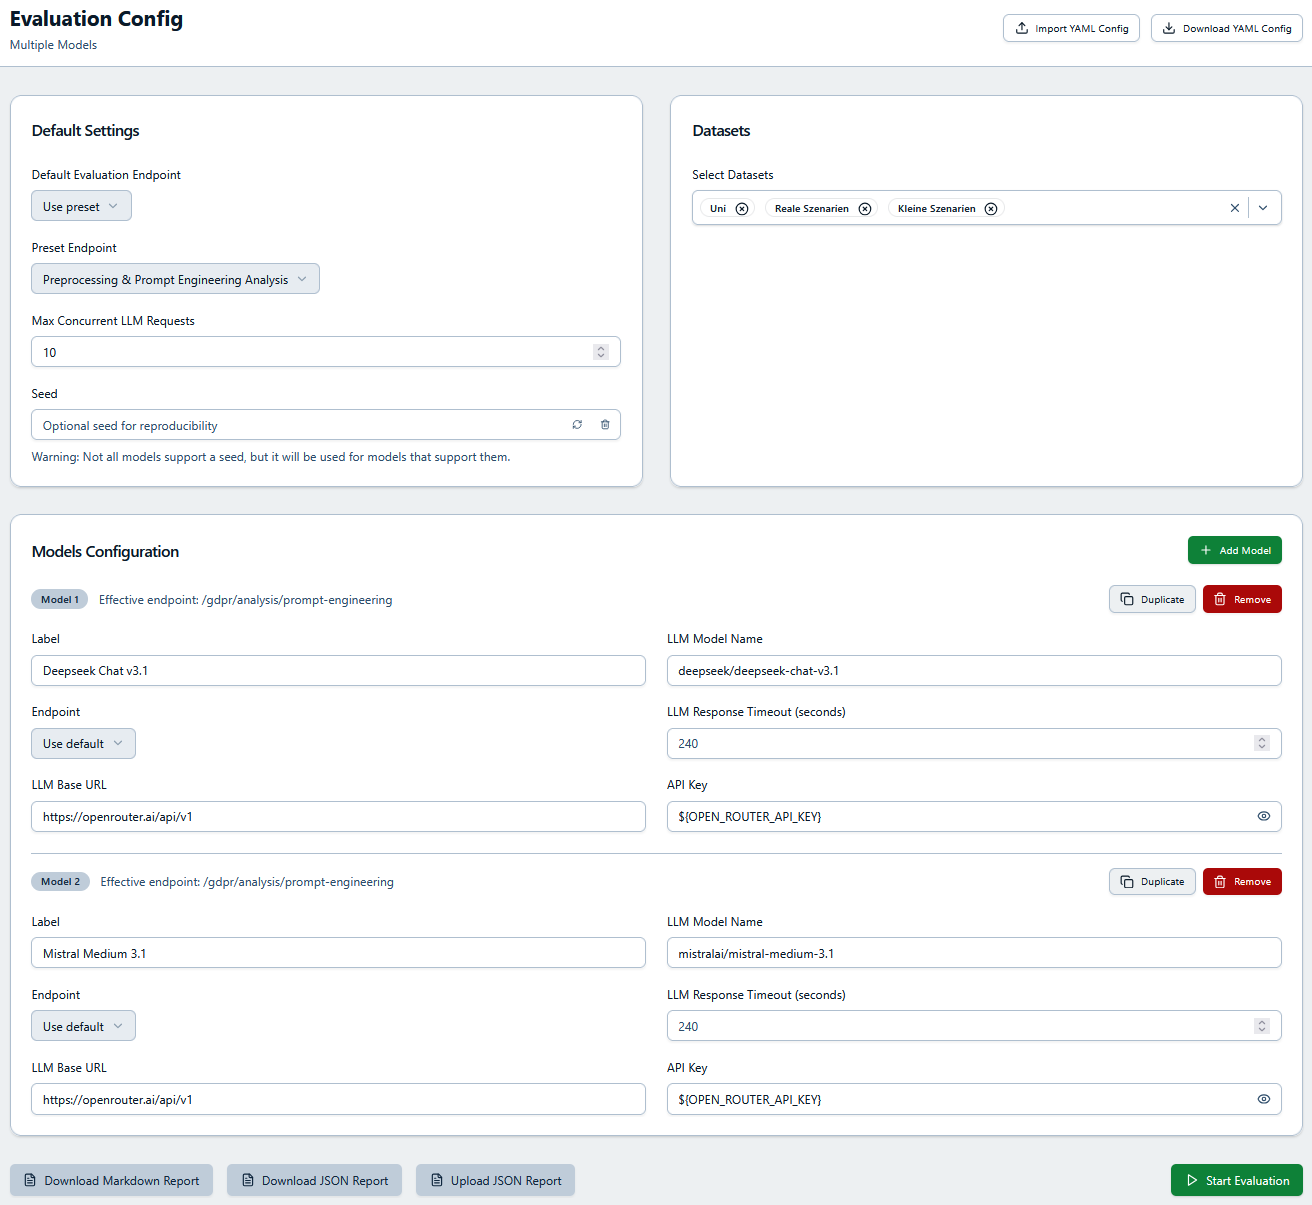
\includegraphics[height=.55\textheight]{images/evaluation/evaluation-config}
    \caption{Formular zur Konfiguration einer Evaluation.}
    \label{fig:evaluation-config}
\end{figure}

\subsection*{Gesamtübersicht}

Nach dem Start der Evaluierung werden die Ergebnisse pro Modell inkrementell vom Backend übermittelt und — wie in Abbildung \ref{fig:evaluation-overview} — angezeigt. Dadurch können Teilergebnisse bereits untersucht werden, während die Evaluierung noch läuft. Die Gesamtübersicht bietet eine kompakte Zusammenfassung pro Modell mit den Kategorien Bestanden, Nicht bestanden und Fehler sowie Side-by-Side-Diagramme aller Metriken mit allen Modellen. So lassen sich die Modelle unmittelbar nebeneinander vergleichen. Oberhalb sind die Metadaten der Evaluierung aufgeführt.

\begin{figure}
    \centering
    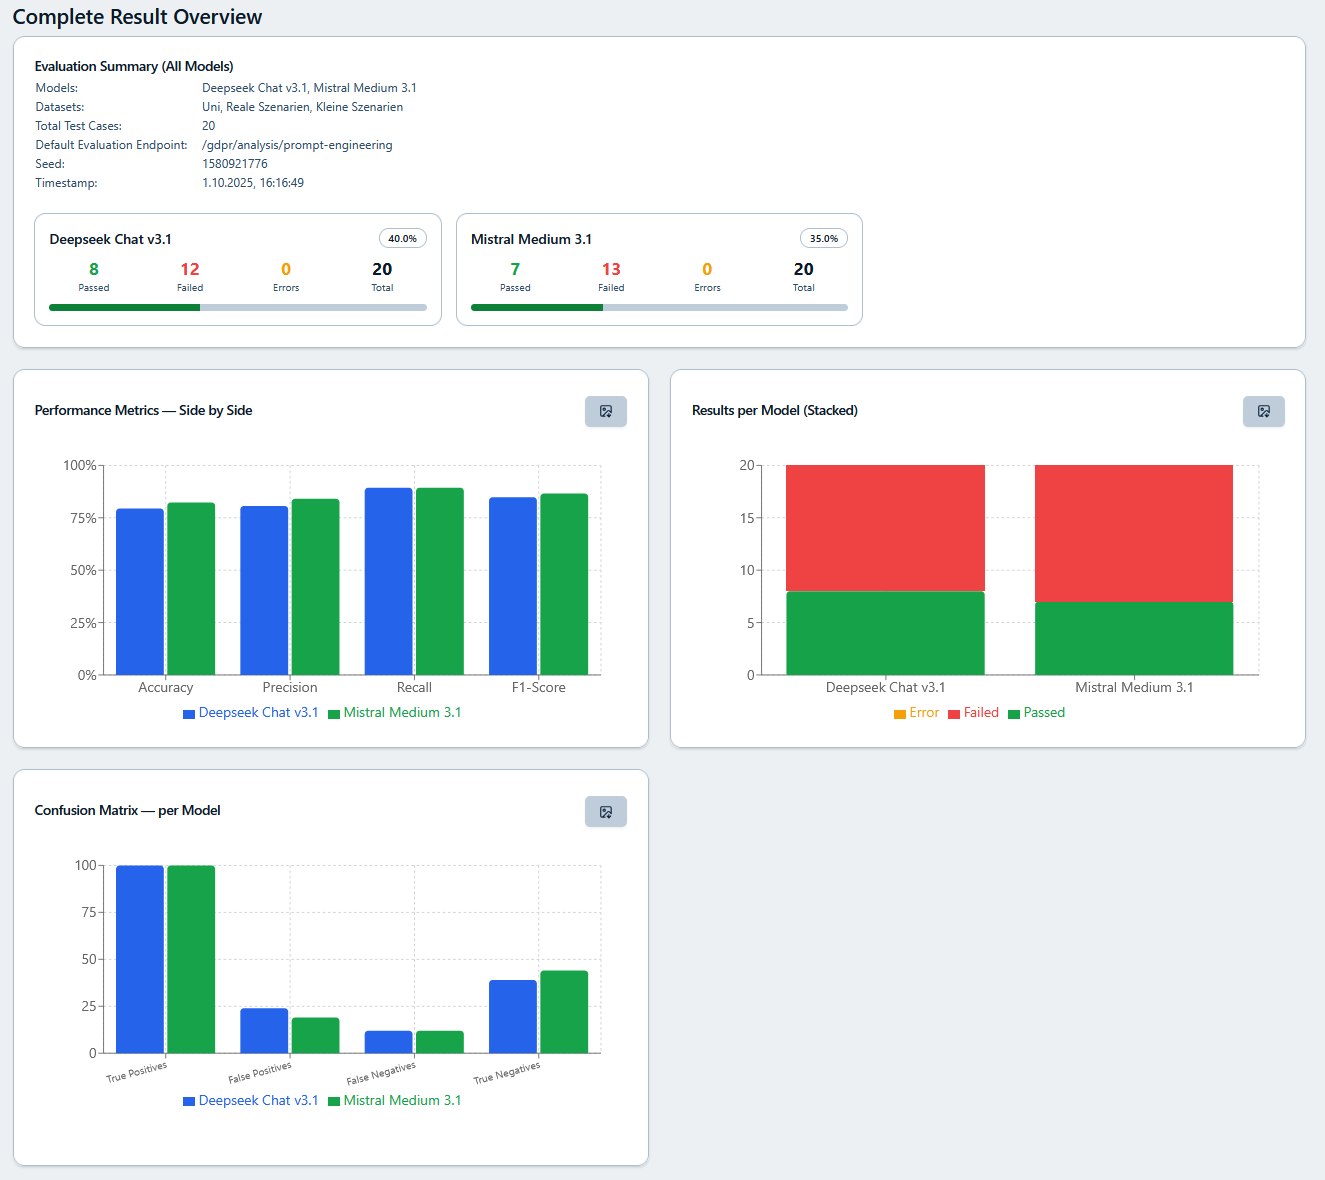
\includegraphics[height=.55\textheight]{images/evaluation/evaluation-result-overview}
    \caption{Gesamtübersicht einer Evaluierung mit Side-by-Side-Diagrammen.}
    \label{fig:evaluation-overview}
\end{figure}

\subsection*{Ergebnisse pro Modell}

Für eine vertiefte Analyse stellt das Frontend für jedes Modell eine Detailansicht bereit, die alle Kennzahlen über sämtliche Testfälle aggregiert. Abbildung \ref{fig:evaluation-by-model} zeigt diese Ansicht. Über Tabs kann zwischen den Modellen gewechselt werden, was einen schnellen Vergleich ermöglicht.

\begin{figure}
    \centering
    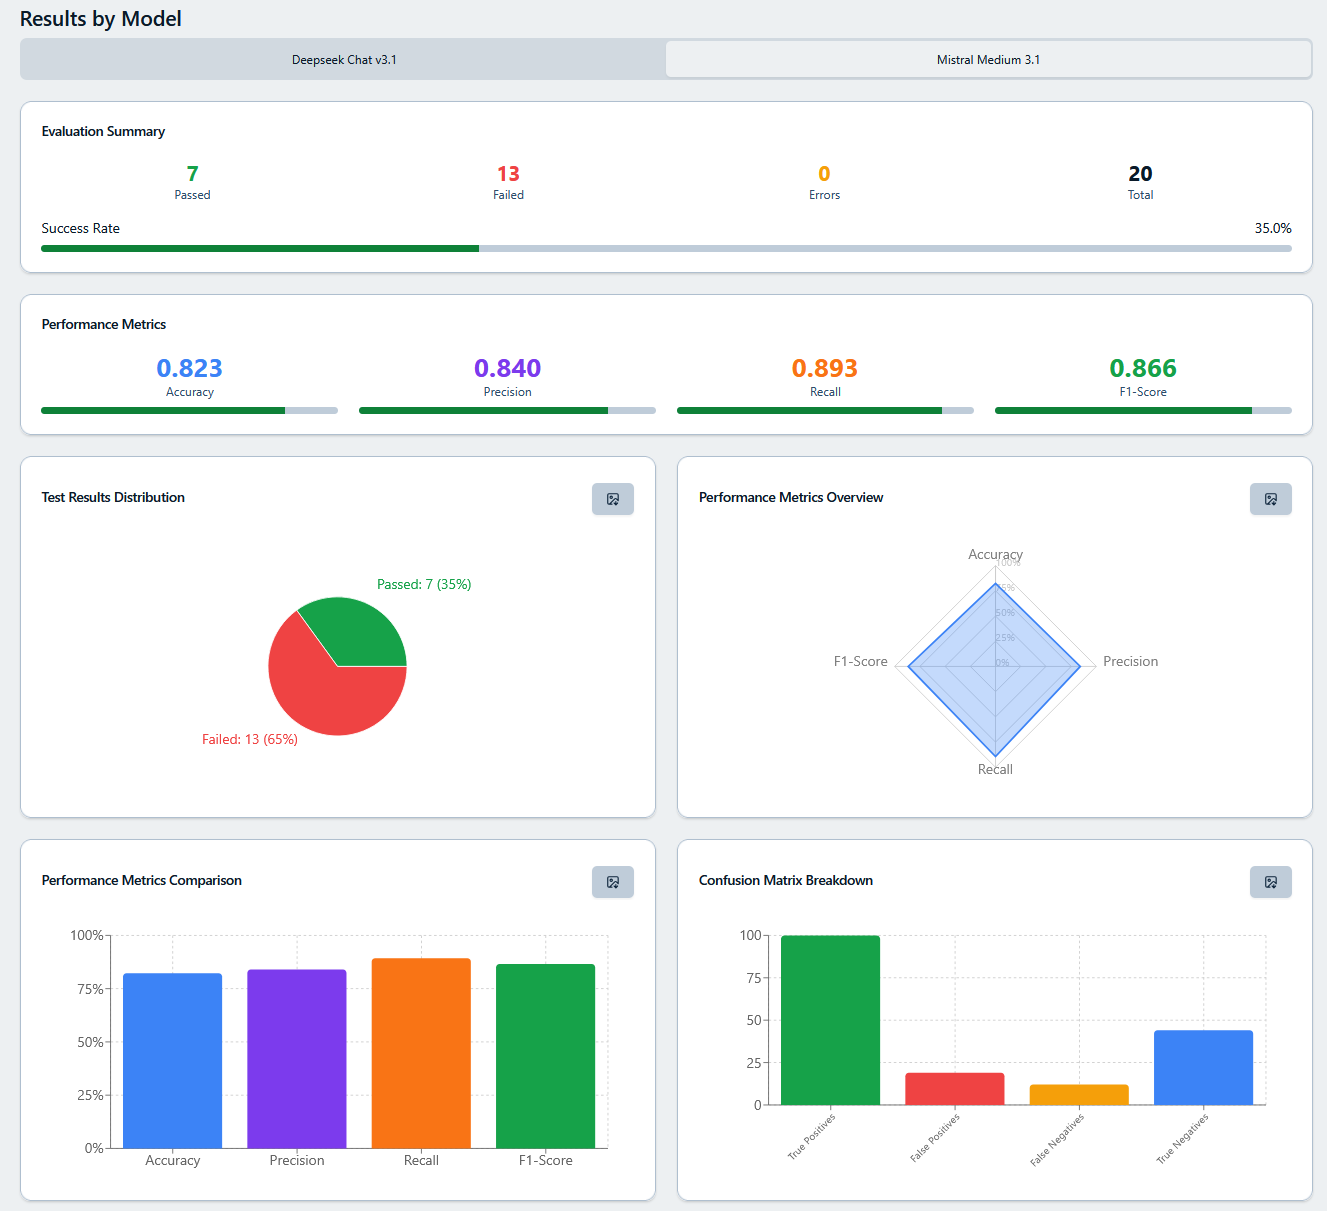
\includegraphics[height=.55\textheight]{images/evaluation/evaluation-result-by-model}
    \caption{Modell-Detailansicht mit exemplarischen Ergebnissen.}
    \label{fig:evaluation-by-model}
\end{figure}

\subsection*{Ergebnisse pro Testfall}

Neben den aggregierten Ergebnissen pro Modell lassen sich auch die Resultate einzelner Testfälle je Modell untersuchen. Abbildung \ref{fig:evaluation-by-testcase} zeigt die Detailseite eines Testfalls. Sie enthält unter anderem den Status, die erwarteten gelabelten Aktivitäten und die vom Modell detektierten Aktivitäten. Zusätzlich visualisiert eine \ac{BPMN}-Darstellung den Prozess, und die Aktivitäten sind je nach korrekter oder inkorrekter Klassifizierung farblich markiert. Falls vorhanden, wird außerdem die vom  \ac{LLM} gelieferte Begründung pro Aktivität angezeigt.

Abweichungen werden dadurch unmittelbar sichtbar, und typische Fehlmuster wie systematische \ac{FP} bei bestimmten Aktivitätstypen lassen sich schnell erkennen. Testfälle, die aufgrund technischer Fehler nicht klassifiziert werden konnten, werden mit der entsprechenden Fehlermeldung aufgeführt.

\begin{figure}
    \centering
    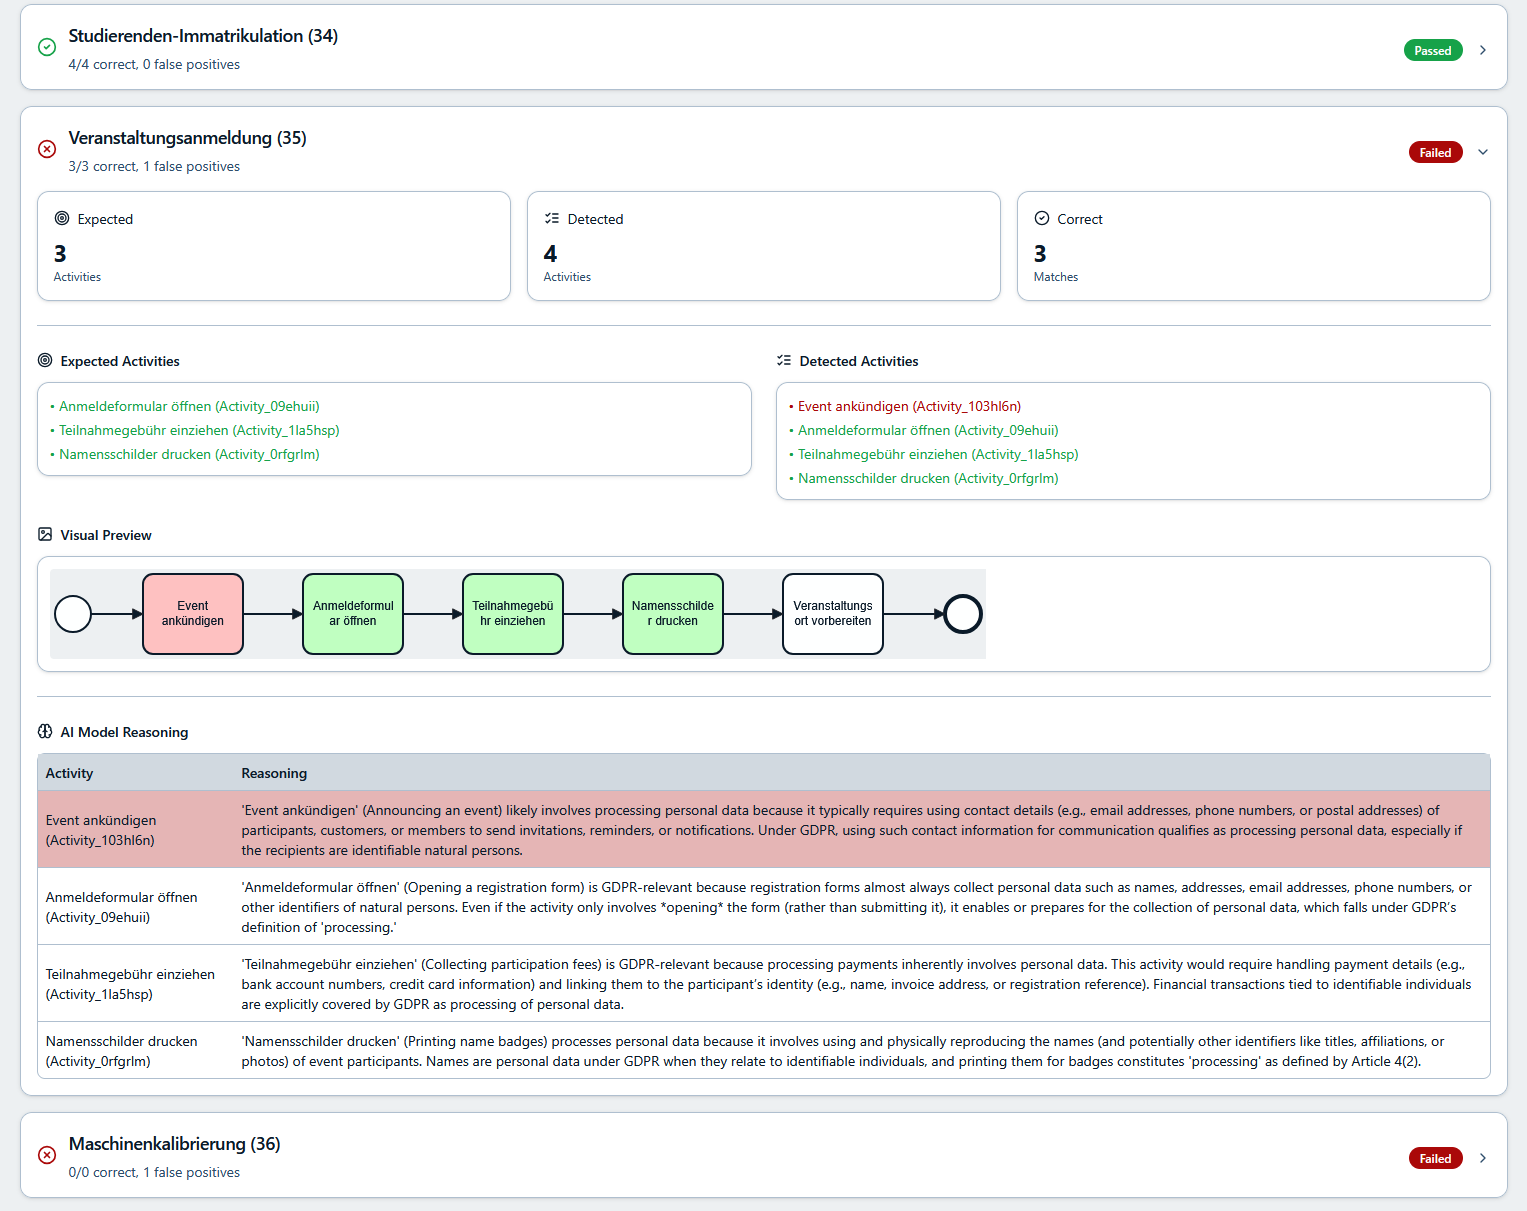
\includegraphics[height=.55\textheight]{images/evaluation/evaluation-result-by-testcase}
    \caption{Detailseite eines Testfalls mit exemplarischen Ergebnissen.}
    \label{fig:evaluation-by-testcase}
\end{figure}.
